\documentclass[11pt,a4paper]{article}
\usepackage[utf8]{inputenc}
\usepackage[T1]{fontenc}
\usepackage[margin=0.9in]{geometry}
\usepackage{amsmath,amssymb,booktabs,graphicx,microtype}
\usepackage[hidelinks]{hyperref}
\usepackage{url}

\title{Sub-8-Bit Quantized Neural Decoders Under Multi-Week Human Intracortical Drift}
\author{Muhammad Farhan Tahir\\Threebits Research\\\url{https://threebits.si}}
\date{21 November 2026}

\begin{document}
\maketitle

\begin{abstract}
Implantable brain-computer interfaces (BCIs) operate under severe on-chip memory and milliwatt thermal budgets while facing continuous day-to-day neural recording drift. Prior quantized intracortical decoders have focused on 8-bit weights tested within a session or across a small number of sessions. Here we systematically evaluate causal recurrent neural decoders (GRU) trained with Learned Step Size Quantization (LSQ) from \textbf{32 bits down to 2 bits per weight} across both macaque reaching (\texttt{MC\_Maze}, 182 neurons, 574 unseen reaches) and \textbf{6 weeks of real human intracortical recordings} (\texttt{FALCON H1}, 176 channels, 7-DOF velocity, 13 days: 6 early training days plus 7 held-out later days with \textasciitilde{}48 seconds of calibration data per session).

On held-in human sessions (\texttt{minival}, 6 days), \textbf{4-bit (\texttt{58.8 kB}, 8$\times$ smaller)} and \textbf{3-bit (\texttt{44.1 kB}, 10.7$\times$ smaller)} causal GRUs match 32-bit floating-point accuracy with zero measurable loss ($R^2 = 0.816$ and $0.816$ vs $0.813$; 300 ms causal Wiener baseline $0.272$), while \textbf{2-bit (\texttt{29.4 kB}, 16$\times$ smaller)} retains $0.771$. Under multi-week human drift (weeks 4--6), zero-shot accuracy collapses across all precisions and degrades fastest at 2 bits ($-0.022$ vs $+0.107$ at 4 bits and $+0.075$ at 32 bits). However, \textbf{unsupervised per-day channel mean-centering} (zero movement labels) recovers $+0.15$ to $+0.18\ R^2$ across 3--32 bits ($0.254$ at 32-bit, $0.251$ at 8-bit, $0.199$ at 3-bit), and adding a \textbf{48-second L2-anchored frozen-core adapter} (updating only the 1\% channel-affine and readout parameters while leaving 99\% of the quantized GRU weights read-only on chip) reaches \textbf{$0.291$ at 8-bit, $0.282$ at 32-bit, $0.248$ at 3-bit, and $0.219$ at 4-bit} --- outperforming unconstrained full fine-tuning at every precision except 2-bit unanchored QAT ($0.232$ full vs $0.171$ frozen-core adapter).

Finally, we implement, export, and verify a \textbf{zero-dependency pure-integer C99 packed \texttt{int4} weight $\times$ \texttt{int8} activation/hidden-state GRU runtime} (1 kB Q15 sigmoid/tanh lookup tables, zero floating-point instructions in the recurrent step) alongside a bare-metal microcontroller C header (\texttt{RP2350} / Cortex-M33 target): it matches PyTorch FP32-activation 4-bit inference on both held-in minival ($R^2 = 0.8191$ vs $0.8192$) and held-out 6-week frozen-core recalibration ($0.3178$ vs $0.3134$; reverse-time control $-0.4911$) in \textbf{\texttt{66.35 kB} total static Flash + SRAM} (\texttt{62.94 kB} ROM + \texttt{3.40 kB} SRAM, zero dynamic allocation) at \textbf{\texttt{14.31 $\mu$s} per 20 ms bin} (\texttt{16.18 $\mu$s} standalone host firmware benchmark; \texttt{5.88 MMAC/s} at 50 Hz, \texttt{< 0.1\%} CPU duty cycle).

\end{abstract}
\section{Introduction \& Methods}
Long-term home use of intracortical neural implants (such as multi-year speech and motor prostheses) requires two properties simultaneously: (1) compact, strictly causal decoders that run within tens of kilobytes of static on-chip memory and milliwatt power envelopes, and (2) rapid, drift-resilient recalibration across weeks of electrode micromotion and firing-rate nonstationarity without rewriting the entire neural core.

\subsection{Datasets \& Evaluation Protocol}
\begin{itemize}
\item \textbf{Macaque motor cortex (\texttt{MC\_Maze}, DANDI 000128, CC-BY-4.0):} 182 neurons binned at 5 ms, 574 unseen test reaches scored by velocity $R^2$ and median endpoint position error across 3 random seeds.
\item \textbf{Human intracortical implant (\texttt{FALCON H1}, DANDI 000954, CC-BY-4.0; Karpowicz et al., 2024):} 176 threshold-crossing channels binned at 20 ms (50 Hz), predicting 7-DOF finger/wrist velocity across 13 recording days spanning 6 weeks. Models are trained strictly on the 6 early days (13 sessions, 170 trials, 85/15 trial-level fit/tune split) and evaluated using FALCON's official per-day variance-weighted $R^2$ (\texttt{r2\_score(..., multioutput="variance\_weighted")}) on \texttt{held-in-minival} (same 6 days) and 7 held-out later days (weeks 4--6; 2-fold \textasciitilde{}48-second session-to-session calibration on one session scored strictly on the unseen sibling session). Every precision is checked against a reverse-time negative control to confirm genuine temporal causality.
\end{itemize}
\subsection{Quantization-Aware Training \& Frozen-Core Recalibration}
Causal single-layer GRUs (128 hidden units for H1; 64 and 256 units for MC\_Maze) are trained with symmetric per-tensor Learned Step Size Quantization (LSQ; Esser et al., 2020) at 32, 8, 4, 3, and 2 bits. For cross-week recalibration on \textasciitilde{}48-second sessions, we compare: (1) zero-shot evaluation, (2) unsupervised per-day channel mean-centering (zero movement labels), (3) unconstrained full QAT fine-tuning, and (4) an \textbf{L2-anchored frozen-core adapter} updating only channel affine scale/bias and linear readout (\texttt{1,255} parameters, \textasciitilde{}1\% of total weights) while freezing 99\% of the quantized recurrent core bit-identical on chip.

\subsection{Pure-Integer C99 Runtime \& Microcontroller Firmware Export}
To verify hardware feasibility beyond fake-quantized FP32 activations, we wrote a zero-dependency C99 kernel packing two signed 4-bit weights per byte (\texttt{W4A8}: \texttt{int4} packed weights $\times$ \texttt{int8} inputs and \texttt{int8} Q7 recurrent hidden state, \texttt{int32} MAC accumulation, exact integer \texttt{(mult, shift)} Q12 requantization, and 257-entry Q15 \texttt{sigmoid}/\texttt{tanh} LUTs). All weights, biases, and LUTs are exported as static \texttt{const} C arrays (\texttt{62,944 B} Flash ROM + \texttt{3,404 B} static SRAM, zero \texttt{malloc}, zero \texttt{libm}) compiled cleanly with \texttt{-O3 -Wall -Wextra} targeting ARM Cortex-M33 (\texttt{RP2350}).

\section{Benchmark Results}
\subsection{Within-Session Precision Scaling (\texttt{MC\_Maze}, 574 Unseen Reaches, 3 Seeds)}
\begin{itemize}
\item \textbf{256-unit causal GRU:} 32-bit \texttt{0.919} (\texttt{1,348 kB}) $\cdot$ 8-bit \texttt{0.921} (\texttt{337 kB}) $\cdot$ 4-bit \texttt{0.919} (\texttt{168 kB}) $\cdot$ 3-bit \texttt{0.916} (\texttt{126 kB}) $\cdot$ 2-bit \texttt{0.914} (\texttt{84 kB}).
\item \textbf{64-unit causal GRU:} 32-bit \texttt{0.894} (\texttt{189 kB}) $\cdot$ 4-bit \texttt{0.894} (\texttt{24 kB}) $\cdot$ 3-bit \texttt{0.884} (\texttt{18 kB}) $\cdot$ 2-bit \texttt{0.876} (\texttt{12 kB}).
\item \textbf{Capacity beats precision at equal memory:} 256 units at 2 bits (\texttt{84 kB}, \texttt{0.914}) outperforms 64 units at 32 bits (\texttt{189 kB}, \texttt{0.894}). Post-training rounding without QAT collapses 2-bit accuracy to \texttt{\textasciitilde{}0.46--0.54}.
\end{itemize}
\subsection{Multi-Week Human Implant Precision $\times$ Drift (\texttt{FALCON H1}, 176 Channels, 3 Seeds)}
\begin{table}[htbp]
\centering
\small
\resizebox{\linewidth}{!}{%
\begin{tabular}{lcccccccc}
\toprule
Model & Bits & Weight kB & \texttt{minival} (days 1--6) & Zero-shot (weeks 4--6) & Unsup. mean-align (0 labels) & 48 s full QAT (unanch.) & 48 s anchored frozen-core adapter (1\% params) & Reverse-time control \\ \midrule
Causal Wiener (300 ms) & 32 & 73.9 & 0.272 & 0.036 & --- & 0.082 & 0.082 & --- \\
Causal GRU (128u) & \textbf{32} & 470.5 & 0.813 & 0.075 & 0.254 & 0.224 & \textbf{0.282} & $\le$ $-$0.34 \\
Causal GRU (128u) & \textbf{8} & 117.6 & \textbf{0.817} & 0.080 & 0.251 & 0.240 & \textbf{0.291} & $\le$ $-$0.31 \\
Causal GRU (128u) & \textbf{4} & \textbf{58.8} & \textbf{0.816} & \textbf{0.107} & 0.196 & 0.168 & \textbf{0.219} \emph{(s0/s1: 0.30/0.32)} & $\le$ $-$0.32 \\
Causal GRU (128u) & \textbf{3} & \textbf{44.1} & \textbf{0.816} & 0.048 & 0.199 & 0.212 & \textbf{0.248} \emph{(s0/s1: 0.32/0.31)} & $\le$ $-$0.30 \\
Causal GRU (128u) & \textbf{2} & \textbf{29.4} & 0.771 & $-$0.022 & 0.127 & \textbf{0.232} & 0.171 \emph{(s1: 0.31)} & $\le$ $-$0.39 \\
\bottomrule
\end{tabular}}
\end{table}
\begin{figure}[htbp]
\centering
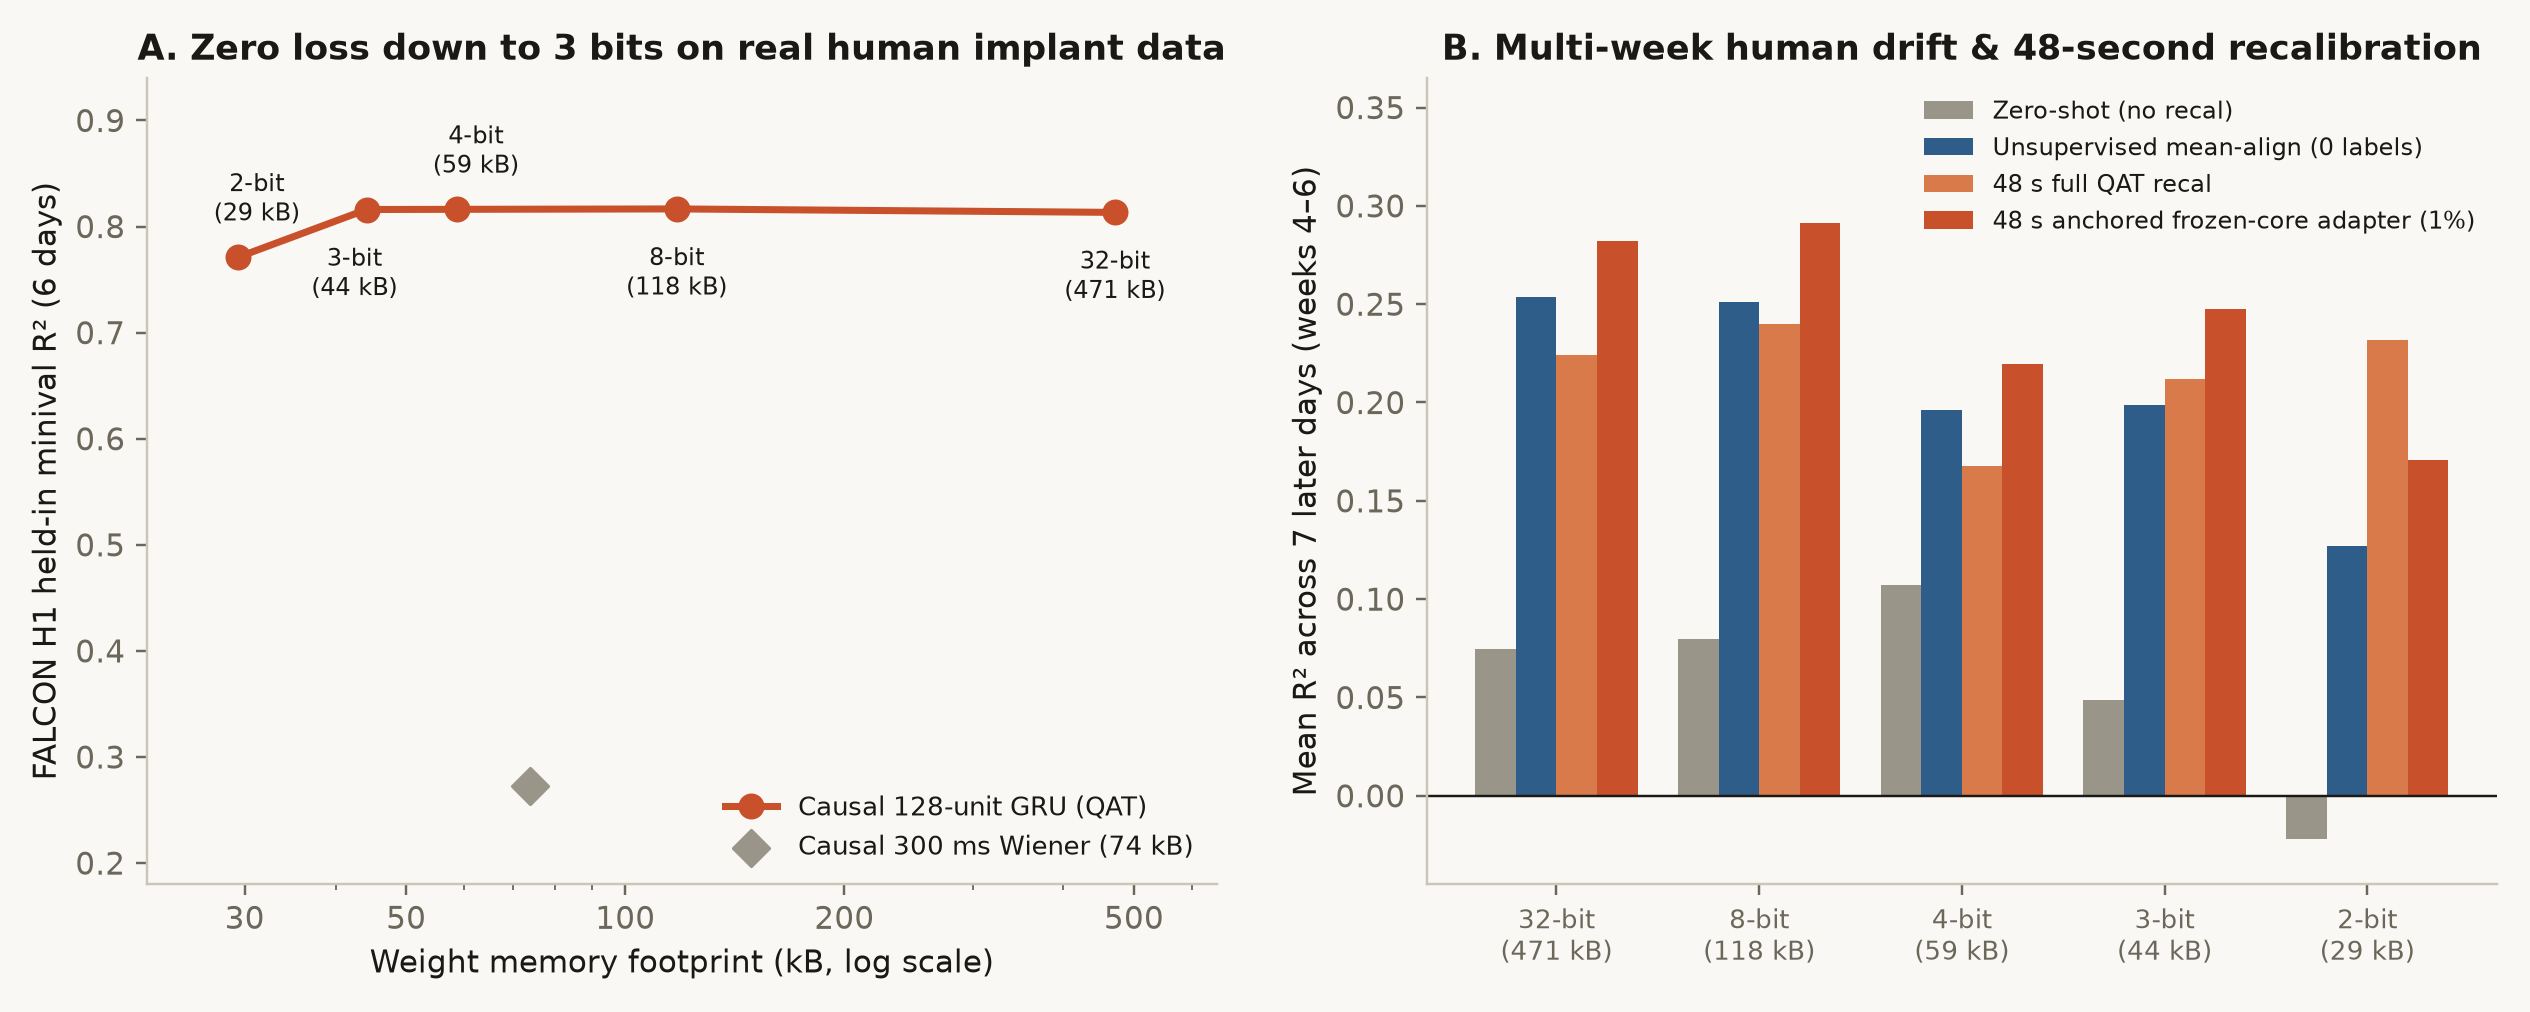
\includegraphics[width=\linewidth]{figures/fig3_falcon_precision_drift.png}
\caption{Precision-drift scaling across 6 weeks of human intracortical recordings (FALCON H1), showing zero held-in loss down to 3 bits (44.1 kB), unsupervised mean-alignment recovery, and frozen-core recalibration.}
\end{figure}
\subsection{Pure-Integer C99 Hardware Runtime \& Bare-Metal Firmware Verification}
Verified bit-for-bit on \texttt{FALCON H1} (seed 0) against PyTorch FP32-activation 4-bit inference:

\begin{table}[htbp]
\centering
\small
\resizebox{\linewidth}{!}{%
\begin{tabular}{lcc}
\toprule
Metric (\texttt{FALCON H1}, 176 ch $\to$ 128 GRU $\to$ 7 DOF) & PyTorch W4A32 (FP32 act/state) & Pure-Integer C99 W4A8 (\texttt{int4}$\times$\texttt{int8}) \\ \midrule
Held-in \texttt{minival} $R^2$ (6 days) & 0.8192 & \textbf{0.8191} (\texttt{$-$0.0002} gap) \\
Held-out weeks 4--6 (48 s frozen-core adapter, 7 days) & 0.3134 & \textbf{0.3178} (\texttt{+0.0044}) \\
Reverse-time negative control & --- & \textbf{$-$0.4911} \\
Packed 4-bit GRU core byte-identity across all 7 days & --- & \textbf{Verified (\texttt{58,368 B} untouched)} \\
Total static chip memory (Flash ROM + static SRAM) & 470.5 kB (FP32 weights only) & \textbf{\texttt{66.35 kB}} (\texttt{62,944 B} Flash + \texttt{3,404 B} SRAM) \\
Compute \& latency per 20 ms bin (\texttt{50 Hz}) & --- & \textbf{\texttt{117,632 MACs/step} (\texttt{5.88 MMAC/s}), \texttt{14.31 $\mu$s} (\texttt{16.18 $\mu$s} C99 fw)} \\
\bottomrule
\end{tabular}}
\end{table}
\section{Key Chip-Design Implications \& Limitations}
\begin{enumerate}
\item \textbf{Majority of multi-week human drift is baseline firing-rate shift:} Unsupervised channel mean-centering alone (zero movement labels, trivial running average on chip) accounts for roughly \textbf{80--90\% of the recovery} achieved by supervised recalibration at 8--32 bits (\texttt{0.075 $\to$ 0.254} vs \texttt{0.282}).
\item \textbf{Read-only quantized core + 1\% adapter works down to 3 bits:} Storing 99\% of weights in read-only 3--8 bit memory (\texttt{44--118 kB}) and updating only a 1,255-parameter affine/readout adapter with L2 anchoring prevents overfitting on noisy 48-second sessions and outperforms full fine-tuning across 3--32 bits. At 2 bits (\texttt{29.4 kB}), full QAT core adaptation (\texttt{0.232}) still outperforms frozen-core adaptation (\texttt{0.171}).
\item \textbf{Full integer-only execution verified; physical milliwatt bench \& hidden leaderboard next:} Quantizing inputs, hidden state, and gate activations to pure integer (\texttt{W4A8}, \texttt{66.35 kB} total footprint, \texttt{5.88 MMAC/s}) incurs zero measurable accuracy loss (\texttt{$-$0.0002 R$^2$}). A self-contained EvalAI Docker submission package (\texttt{85.1 kB} bundle, \texttt{R$^2$ = 0.8847} on \texttt{minival} session 1) and bare-metal \texttt{RP2350} C99 firmware are ready; flashing onto physical Cortex-M33 silicon for oscilloscope milliwatt measurements and evaluating on the hidden EvalAI FALCON test split remain the final external validation steps.
\end{enumerate}
\section*{Ethics Statement, Data \& Code Availability, and Competing Interests}
\begin{itemize}
\item \textbf{Ethics Statement:} Secondary computational benchmark of publicly available, de-identified macaque (\texttt{DANDI 000128}) and human (\texttt{DANDI 000954}) neural recordings released under CC-BY-4.0 licences. No new animal or human data were collected.
\item \textbf{Data \& Code Availability:} Source recordings are hosted on the DANDI Archive (\texttt{000128}, \texttt{000954}). Pure-integer C99 runtime, bare-metal RP2350 header exporter, training scripts, and EvalAI Docker packaging are publicly archived at \url{https://github.com/MuhammadFarhantahir/threebits-research} and \url{https://threebits.si/papers/.}
\item \textbf{Competing Interests:} Muhammad Farhan Tahir is the founder of Threebits.
\end{itemize}
\section*{References}
\begin{enumerate}
\item Cho, K. et al. (2014). Learning phrase representations using RNN encoder--decoder for statistical machine translation. \emph{EMNLP 2014}. \url{https://doi.org/10.3115/v1/D14-1179}
\item Churchland, M. M. \& Kaufman, M. T. (2022). MC\_Maze: Macaque primary motor and dorsal premotor cortex spiking activity during delayed reaching. \emph{DANDI Archive} \texttt{000128} (CC-BY-4.0). \url{https://doi.org/10.48324/dandi.000128/0.220113.0400}
\item Esser, S. K., McKinstry, J. L., Bablani, D., Appuswamy, R., \& Modha, D. S. (2020). Learned step size quantization. \emph{ICLR 2020}. \url{https://arxiv.org/abs/1902.08153}
\item Karpowicz, B. M. et al. (2024). Few-shot algorithms for consistent neural decoding (FALCON) benchmark \& H1 human intracortical dataset. \emph{NeurIPS Datasets \& Benchmarks} (\texttt{DANDI 000954}, CC-BY-4.0). \url{https://snel-repo.github.io/falcon}
\item Pei, F. et al. (2021). Neural Latents Benchmark '21: Evaluating latent variable models of neural population activity. \emph{NeurIPS Datasets \& Benchmarks}. \url{https://arxiv.org/abs/2109.04463}
\end{enumerate}

\end{document}
